\chapter{Chromatografie}\label{ch:b2:chromatography}

Een druppel energiedrank, verdund en gefiltreerd, wordt geïnjecteerd in een stalen buisje dat niet langer is dan een pen en
gevuld is met silicakorrels van enkele micrometer. Een paar minuten later heeft een detector een lijn getekend
met een handvol pieken, en uit de oppervlakte van een ervan meldt het laboratorium hoeveel cafeïne het
blikje bevat, op enkele procenten na. \omterm{def:b2:chromatography:principle}{Chromatografie} scheidt de componenten van een mengsel door ze
met verschillende snelheden door een kolom te laten racen; dit hoofdstuk legt uit waarom ze verschillend snel gaan,
waarom hun pieken de breedte hebben die ze hebben, hoe je twee buren scheidt, en hoe je van een piek
een hoeveelheid maakt.

\begin{omfigure}
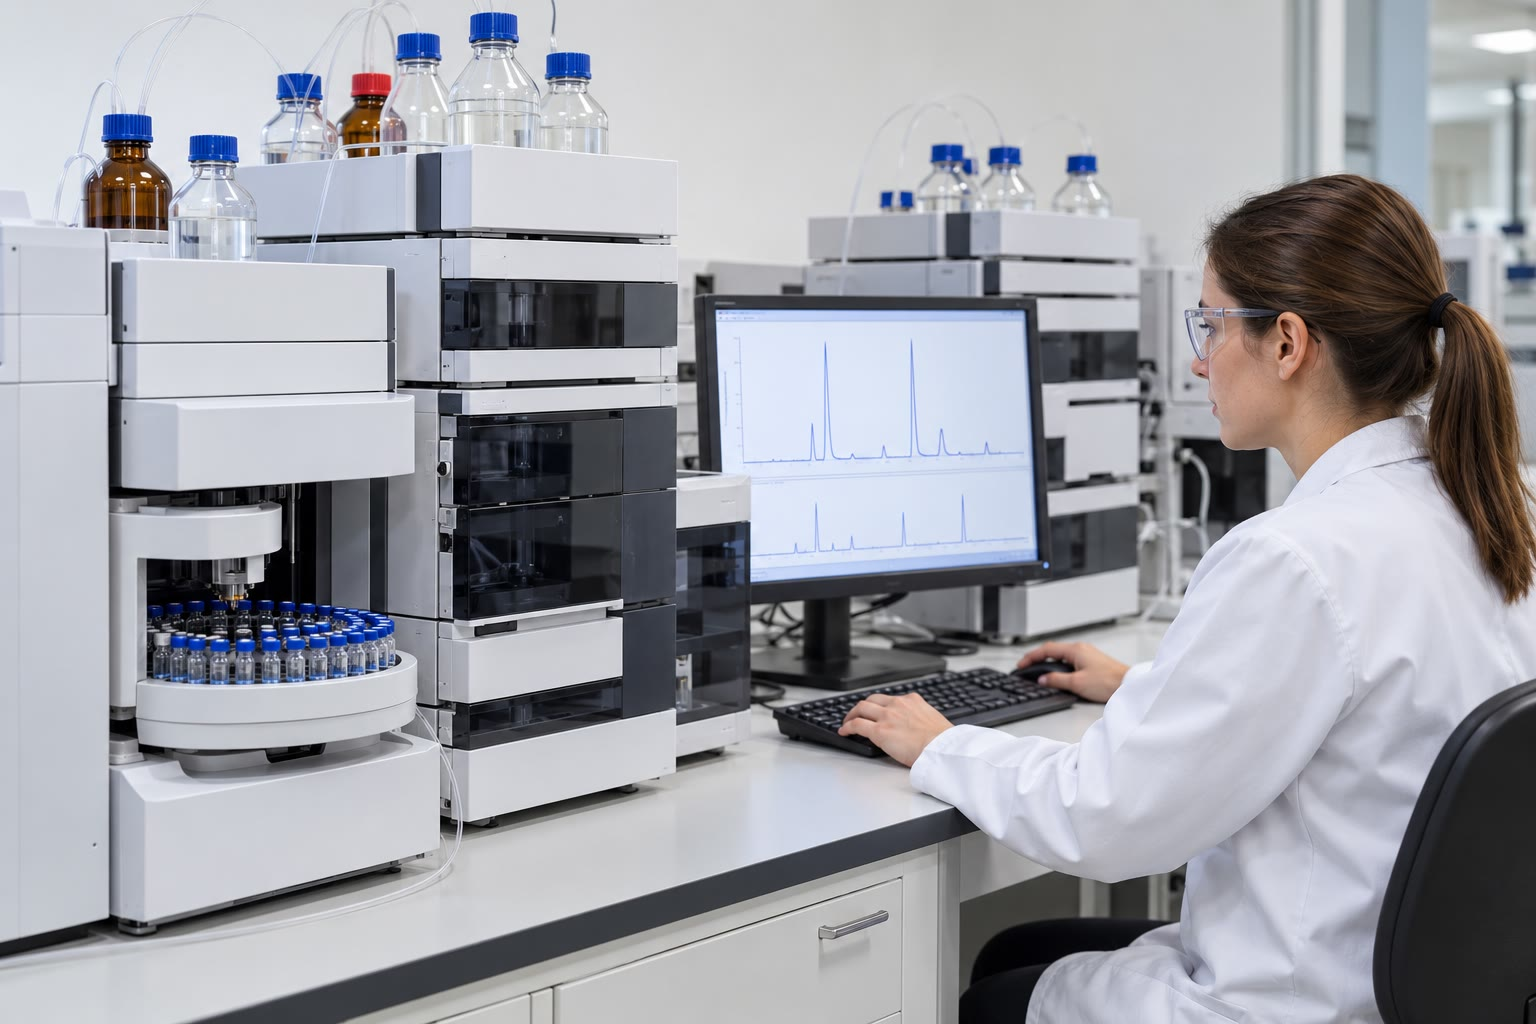
\includegraphics[width=0.58\linewidth]{images/book3/ai/b2-31-analytical-lab.jpg}

{\small Een analytisch laboratorium: vloeistofchromatografen met hun oplosmiddelflessen en een autosamplerplateau
met flesjes; de chromatogrammen verschijnen op het scherm (illustratie).}
\end{omfigure}

\begin{recall}
Het schoolboek: papier- en dunnelaagchromatografie, chromatogram, loopvloeistof. Het deel van jaar~1: de
verdelingscoëfficiënt, vloeistof-vloeistofextractie, de retentiefactor $R_f$ van een dunnelaagplaat.
\Cref{ch:b2:liquid-vapour-diagrams}: de \omterm{def:b2:liquid-vapour-diagrams:fractional-distillation}{theoretische schotel} van een destillatiekolom.
\end{recall}

\section{Principe}

\begin{definition}[Chromatografie]\label{def:b2:chromatography:principle}
\emph{Chromatografie}\index{chromatografie} scheidt de componenten van een mengsel door ze te verdelen
tussen een \emph{stationaire fase}\index{stationaire fase}, vastgezet in een kolom of op een plaat, en een
\emph{mobiele fase}\index{mobiele fase}, een gas of een vloeistof die erlangs stroomt. Het meevoeren van de componenten
door en uit de kolom met de mobiele fase is \emph{elutie}\index{elutie}.
\end{definition}

Een molecuul beweegt alleen zolang het in de \omterm{def:b2:chromatography:principle}{mobiele fase} is; zolang de \omterm{def:b2:chromatography:principle}{stationaire fase} het vasthoudt,
wacht het. Het wisselt onderweg miljoenen keren tussen de twee fasen, dus zijn gemiddelde snelheid wordt bepaald door
de fractie van de tijd die het in elk ervan doorbrengt, dat wil zeggen door zijn verdelingsevenwicht.

\begin{definition}[Retentie]\label{def:b2:chromatography:retention}
De \emph{retentietijd}\index{retentietijd} $t_R$ van een verbinding is de tijd van de injectie tot het
maximum van haar piek; de \emph{dode tijd}\index{dode tijd} $t_M$ is de retentietijd van een
niet-weerhouden verbinding, die nooit in de \omterm{def:b2:chromatography:principle}{stationaire fase} komt. De \emph{retentiefactor}\index{retentiefactor k@retentiefactor $k$}
$k$ van een verbinding op een kolom is
\begin{equation*}
k = \frac{t_R - t_M}{t_M}.
\end{equation*}
Het is niet de $R_f$ van een dunnelaagplaat, die een afgelegde afstand meet, al beschrijven beide
dezelfde verdeling.
\end{definition}

\begin{proposition}[Retentietijd]\label{prop:b2:chromatography:retention-time}
Als de hoeveelheden van een verbinding in de stationaire en de \omterm{def:b2:chromatography:principle}{mobiele fase} van een plakje kolom bij evenwicht
$n_s$ en $n_m$ zijn, beweegt de verbinding met $u/(1 + n_s/n_m)$, waarin $u$ de snelheid van de \omterm{def:b2:chromatography:principle}{mobiele fase} is,
en is $t_R = t_M(1 + n_s/n_m)$.
\end{proposition}

\begin{proof}
Een gegeven molecuul brengt de fractie $n_m/(n_s + n_m)$ van zijn tijd door in de \omterm{def:b2:chromatography:principle}{mobiele fase}, waar het beweegt met
$u$, en de rest in rust. Zijn gemiddelde snelheid is $u\,n_m/(n_s + n_m) = u/(1 + n_s/n_m)$. De kolom met
lengte $L$ wordt doorlopen in $t_R = (L/u)(1 + n_s/n_m)$, en $L/u = t_M$.
\end{proof}

\begin{proposition}[Retentie en verdeling]\label{prop:b2:chromatography:k-and-K}
De \omterm{def:b2:chromatography:retention}{retentiefactor} is de verhouding van de hoeveelheden in de twee fasen, $k = n_s/n_m = KV_s/V_m$, waarin $K$
de verdelingscoëfficiënt is (concentratie in de \omterm{def:b2:chromatography:principle}{stationaire fase} gedeeld door concentratie in de \omterm{def:b2:chromatography:principle}{mobiele
fase}) en $V_s$, $V_m$ de volumes van de fasen in de kolom.
\end{proposition}

\begin{proof}
Uit \cref{prop:b2:chromatography:retention-time} volgt $(t_R - t_M)/t_M = n_s/n_m$. Met $n_s = c_sV_s$,
$n_m = c_mV_m$ en $K = c_s/c_m$ is $n_s/n_m = KV_s/V_m$.
\end{proof}

Twee verbindingen scheiden als hun verdelingscoëfficiënten verschillen; de kolomgeometrie ($V_s/V_m$)
vermenigvuldigt alle retenties op dezelfde manier. De \omterm{def:b2:chromatography:principle}{mobiele fase} veranderen, wat $K$ verandert, is de belangrijkste
hefboom van de chemicus op de retentie.

\begin{omfigure}
\begin{tikzpicture}[x=1cm, y=1cm]
\foreach \x/\a/\b/\ha/\hb/\lab in {0/0.6/0.6/0.1/0.1/begin, 2.4/1.5/2.6/0.16/0.22/later, 4.8/2.4/4.4/0.2/0.3/einde}{
  \draw[black!60] (\x-0.35,0) rectangle (\x+0.35,-5);
  \fill[omThm!55] (\x-0.33,-\b+\hb) rectangle (\x+0.33,-\b-\hb);
  \fill[omDef!55, opacity=0.85] (\x-0.33,-\a+\ha) rectangle (\x+0.33,-\a-\ha);
  \node[font=\small] at (\x,-5.4) {\lab};
}
\draw[->, thick] (-1.0,-0.3) -- (-1.0,-4.6) node[midway, left, font=\small, align=right] {mobiele\\fase};
\node[font=\small, align=left, anchor=west] at (5.5,-2.4) {sterker weerhouden\\(traag, smal)};
\node[font=\small, align=left, anchor=west] at (5.5,-4.4) {minder weerhouden\\(snel)};
\draw[densely dotted] (5.15,-2.4) -- (5.5,-2.4); \draw[densely dotted] (5.15,-4.4) -- (5.5,-4.4);
\end{tikzpicture}
\par\vspace{4pt}

{\small Twee verbindingen die samen als één dunne band geïnjecteerd zijn, bewegen door een kolom (drie momentopnamen,
schematisch). De minst weerhouden verbinding (kleinere $k$) loopt voorop; beide banden worden breder onderweg, die
welke het verst gekomen is het meest.}
\end{omfigure}

\section{Piekbreedte en schotelgetal}

Een band blijft niet dun. Moleculen van dezelfde verbinding volgen verschillende wegen tussen de korrels,
diffunderen langs de kolom en blijven willekeurig lang achter in de \omterm{def:b2:chromatography:principle}{stationaire fase}. De piek die aan
de uitgang geregistreerd wordt, is zeer nauwkeurig een gaussfunctie met standaardafwijking $\sigma_t$ (in tijd), en hoe smaller hij is
bij een gegeven $t_R$, hoe beter de kolom.

\begin{definition}[Schotelgetal]\label{def:b2:chromatography:plates}
Het \emph{schotelgetal}\index{schotelgetal} van een kolom voor een verbinding is $N = (t_R/\sigma_t)^2$, waarin
$\sigma_t$ de standaardafwijking van haar piek in tijd is. De \emph{schotelhoogte}\index{schotelhoogte} is
$H = L/N$, voor een kolom met lengte $L$.
\end{definition}

De namen komen van de destillatiekolom van \cref{ch:b2:liquid-vapour-diagrams}: een chromatografische
kolom gedraagt zich alsof ze een stapel van $N$ evenwichtstrappen was, elk $H$ hoog. De analogie is een manier van
tellen, geen beeld van de kolom.

\begin{proposition}[Schotelgetal uit een piek]\label{prop:b2:chromatography:plate-number}
Met $w$ de basisbreedte tussen de raaklijnen in de buigpunten en $w_{1/2}$ de breedte op
halve hoogte geldt
\begin{equation*}
N = 16\left(\frac{t_R}{w}\right)^2 = 5.54\left(\frac{t_R}{w_{1/2}}\right)^2.
\end{equation*}
\end{proposition}

\begin{proof}
Voor een gaussfunctie met standaardafwijking $\sigma$ en hoogte $h$ liggen de buigpunten op $\pm\sigma$,
waar de hoogte $h\mathrm e^{-1/2}$ is en de helling $\mp h\mathrm e^{-1/2}/\sigma$; de raaklijn daar
bereikt nul na nog eens $\sigma$, op $\pm2\sigma$: $w = 4\sigma$. De halve hoogte wordt bereikt waar
$\mathrm e^{-x^2/2\sigma^2} = 1/2$, $x = \sigma\sqrt{2\ln2}$: $w_{1/2} = 2\sqrt{2\ln2}\,\sigma \approx
2.355\,\sigma$. Invullen van $\sigma = w/4$ of $\sigma = w_{1/2}/2.355$ in $N = (t_R/\sigma)^2$ geeft
$16$ en $2.355^2 = 5.545$, geschreven als 5.54.
\end{proof}

\begin{proposition}[Vergelijking van Van Deemter]\label{prop:b2:chromatography:van-deemter}
De \omterm{def:b2:chromatography:plates}{schotelhoogte} hangt als volgt af van de lineaire snelheid $u$ van de \omterm{def:b2:chromatography:principle}{mobiele fase}:
\begin{equation*}
H = A + \frac{B}{u} + Cu,
\end{equation*}
waarin $A$ staat voor de verschillende wegen door de pakking, $B/u$ voor diffusie langs de kolom
(erger wanneer de moleculen langer blijven) en $Cu$ voor de trage uitwisseling met de \omterm{def:b2:chromatography:principle}{stationaire fase} (erger
wanneer de \omterm{def:b2:chromatography:principle}{mobiele fase} voorbijjaagt). $H$ is het kleinst bij $u_{\mathrm{opt}} = \sqrt{B/C}$, waar $H_{\min} =
A + 2\sqrt{BC}$.
\end{proposition}

\admitted

De vorm van de vergelijking wordt aangenomen; haar minimum niet. $\mathrm dH/\mathrm du = -B/u^2 + C$ wordt nul
bij $u = \sqrt{B/C}$, en daar is $B/u = Cu = \sqrt{BC}$, dus $H_{\min} = A + 2\sqrt{BC}$; de tweede
afgeleide $2B/u^3$ is positief, dus dit is een minimum. Kleine korrels verkleinen $A$ en $C$: daarom
gebruikt moderne vloeistofchromatografie deeltjes van enkele micrometer en hoge drukken om de \omterm{def:b2:chromatography:principle}{mobiele
fase} erdoor te duwen.

\begin{omfigure}
\begin{tikzpicture}
\begin{axis}[width=0.7\linewidth, height=5.2cm, xmin=0, xmax=8, ymin=0, ymax=70,
  xlabel={lineaire snelheid $u$ (\unit{mm/s})}, ylabel={schotelhoogte $H$ (\unit{\micro m})},
  label style={font=\small}, tick label style={font=\scriptsize},
  legend style={font=\scriptsize, at={(1.03,1)}, anchor=north west}, legend cell align=left]
\addplot[omDef, very thick] table[x=u, y=H] {figdata/out/bachelor-2-chromatogram-b.dat};
\addplot[black!50, dashed] table[x=u, y=A] {figdata/out/bachelor-2-chromatogram-b.dat};
\addplot[omThm, dashed] table[x=u, y=B] {figdata/out/bachelor-2-chromatogram-b.dat};
\addplot[omMeth, dashed] table[x=u, y=C] {figdata/out/bachelor-2-chromatogram-b.dat};
\addplot[only marks, mark=*, mark size=1.6pt] coordinates {(2,30)};
\legend{$H$, $A$, $B/u$, $Cu$}
\end{axis}
\end{tikzpicture}

{\small Een van-deemterkromme (parameters voor de oefening: $A = \qty{10}{\micro m}$, $B = \qty{20}{\micro m.mm/s}$,
$C = \qty{5}{\micro m.s/mm}$). Het minimum, $H = \qty{30}{\micro m}$ bij $u = \qty{2}{mm/s}$, ligt waar
de diffusie- en de uitwisselingsterm gelijk zijn.}
% figdata: bachelor-2/chromatogram.py part b
\end{omfigure}

\section{Twee verbindingen scheiden}

\begin{definition}[Selectiviteit en resolutie]\label{def:b2:chromatography:separation}
Voor twee naburige pieken met $k_2 > k_1$ is de \emph{selectiviteitsfactor}\index{selectiviteitsfactor}
$\alpha = k_2/k_1$, en de \emph{resolutie}\index{resolutie}
\begin{equation*}
R_s = \frac{2(t_{R2} - t_{R1})}{w_1 + w_2},
\end{equation*}
de afstand tussen de pieken gedeeld door hun gemiddelde basisbreedte.
\end{definition}

Bij $R_s = 1$ overlappen de pieken nog zichtbaar; bij $R_s = 1.5$ keert het signaal tussen
hen terug naar de basislijn (basislijnscheiding), wat het gebruikelijke doel is voor kwantitatief werk.

\begin{omfigure}
\begin{tikzpicture}
\begin{axis}[width=0.36\linewidth, height=3.6cm, xmin=-8, xmax=8, ymin=0, ymax=1.15,
  xtick=\empty, ytick=\empty, axis x line=bottom, axis y line=none, title style={font=\small},
  title={$R_s = 0.75$}]
\addplot[omDef, thick] table[x=x, y=r075] {figdata/out/bachelor-2-chromatogram-a.dat};
\end{axis}
\end{tikzpicture}\hfill\begin{tikzpicture}
\begin{axis}[width=0.36\linewidth, height=3.6cm, xmin=-8, xmax=8, ymin=0, ymax=1.15,
  xtick=\empty, ytick=\empty, axis x line=bottom, axis y line=none, title style={font=\small},
  title={$R_s = 1.0$}]
\addplot[omDef, thick] table[x=x, y=r100] {figdata/out/bachelor-2-chromatogram-a.dat};
\end{axis}
\end{tikzpicture}\hfill\begin{tikzpicture}
\begin{axis}[width=0.36\linewidth, height=3.6cm, xmin=-8, xmax=8, ymin=0, ymax=1.15,
  xtick=\empty, ytick=\empty, axis x line=bottom, axis y line=none, title style={font=\small},
  title={$R_s = 1.5$}]
\addplot[omDef, thick] table[x=x, y=r150] {figdata/out/bachelor-2-chromatogram-a.dat};
\end{axis}
\end{tikzpicture}

{\small Twee gaussische pieken van gelijke grootte bij drie \omterm{def:b2:chromatography:separation}{resoluties} (model). Bij 0.75 versmelten ze tot een
doublet; bij 1.0 ligt het dal nog op een kwart van de hoogte; bij 1.5 is het signaal terug op de
basislijn.}
% figdata: bachelor-2/chromatogram.py part a
\end{omfigure}

\begin{theorem}[Resolutievergelijking]\label{thm:b2:chromatography:resolution}
Voor twee naburige pieken met hetzelfde \omterm{def:b2:chromatography:plates}{schotelgetal} $N$ geldt
\begin{equation*}
R_s = \frac{\sqrt N}{4}\,\frac{\alpha - 1}{\alpha}\,\frac{k_2}{1 + k_2}.
\end{equation*}
\end{theorem}

\begin{proof}
Bij pieken die dicht bij elkaar liggen, zijn de twee basisbreedten bijna gelijk; neem ze allebei gelijk aan die van de tweede piek,
$w = 4\sigma_t = 4t_{R2}/\sqrt N$ (\cref{def:b2:chromatography:plates}). Dan is $R_s = (t_{R2} -
t_{R1})/w = \sqrt N\,(t_{R2} - t_{R1})/(4t_{R2})$. Met $t_R = t_M(1 + k)$
(\cref{prop:b2:chromatography:retention-time}) is $t_{R2} - t_{R1} = t_M(k_2 - k_1)$ en $t_{R2} =
t_M(1 + k_2)$, dus $R_s = (\sqrt N/4)(k_2 - k_1)/(1 + k_2)$. Ten slotte is $k_2 - k_1 = k_2(1 - 1/\alpha) =
k_2(\alpha - 1)/\alpha$.
\end{proof}

\begin{method}[Een resolutie verbeteren]\label{met:b2:chromatography:improve-resolution}
\begin{enumerate}
  \item Efficiëntie: $R_s \propto \sqrt N$. De kolomlengte verdubbelen verdubbelt $N$ en de analysetijd,
        maar vermenigvuldigt $R_s$ maar met $\sqrt2 \approx 1.41$; kleinere deeltjes of het optimale debiet
        verhogen $N$ bij constante lengte.
  \item Selectiviteit: de factor $(\alpha - 1)/\alpha$ is het gevoeligst. Verander de \omterm{def:b2:chromatography:principle}{mobiele fase}
        (oplosmiddel, pH), de \omterm{def:b2:chromatography:principle}{stationaire fase} of, bij \omterm{def:b2:chromatography:techniques}{gaschromatografie}, de temperatuur.
  \item Retentie: $k_2/(1+k_2)$ stijgt steil tot $k \approx 2$ en daarna langzaam, terwijl de tijd
        blijft toenemen als $1 + k$; mik op een $k$ tussen ongeveer 2 en 10.
\end{enumerate}
\end{method}

\section{Technieken}

\begin{definition}[Chromatografische technieken]\label{def:b2:chromatography:techniques}
Bij \emph{gaschromatografie}\index{gaschromatografie} (GC) is de \omterm{def:b2:chromatography:principle}{mobiele fase} een gas (helium, waterstof
of stikstof) en de \omterm{def:b2:chromatography:principle}{stationaire fase} een vloeistoffilm op de binnenwand van een lange capillaire kolom, die
in een oven staat. Bij \emph{hogedrukvloeistofchromatografie}\index{hogedrukvloeistofchromatografie}
(HPLC) duwt een pomp een vloeibare \omterm{def:b2:chromatography:principle}{mobiele fase} door een korte kolom die gepakt is met kleine
deeltjes. Bij HPLC met \emph{omgekeerde fase}\index{omgekeerde fase} is de \omterm{def:b2:chromatography:principle}{stationaire fase} apolair
(silica met lange alkylketens) en de \omterm{def:b2:chromatography:principle}{mobiele fase} een polair mengsel van water met methanol of
acetonitril. Bij \emph{gradiëntelutie}\index{gradientelutie@gradiëntelutie} wordt de samenstelling van de \omterm{def:b2:chromatography:principle}{mobiele fase}
tijdens de run veranderd, bij vloeistofchromatografie, om sterk weerhouden verbindingen sneller te elueren.
\end{definition}

\begin{omfigure}
\begin{tikzpicture}[x=1cm, y=1cm, box/.style={draw=black!70, rounded corners=2pt, fill=white,
  font=\small, align=center, minimum height=0.8cm, inner sep=3pt}]
\node[box] (gas) at (0,0) {draag-\\gas};
\node[box] (inj) at (2.2,0) {verwarmde\\injector};
\draw[black!70, rounded corners=2pt, fill=omDef!8] (3.5,-1.1) rectangle (6.5,1.1);
\node[font=\small] at (5,0.85) {oven};
\draw[omDef, thick] (5,-0.15) circle (0.55); \draw[omDef, thick] (5,-0.15) circle (0.42);
\node[box] (det) at (8.0,0) {detector};
\node[box] (data) at (10.2,0) {data-\\systeem};
\draw[->, thick] (gas) -- (inj);
\draw[->, thick] (inj.east) -- (4.45,0);
\draw[->, thick] (5.55,0) -- (det.west);
\draw[->, thick] (det) -- (data);
\node[font=\footnotesize, align=center] at (5,-1.45) {capillaire kolom (opgerold)};
\end{tikzpicture}

\medskip
\begin{tikzpicture}[x=1cm, y=1cm, box/.style={draw=black!70, rounded corners=2pt, fill=white,
  font=\small, align=center, minimum height=0.8cm, inner sep=3pt}]
\node[box] (sol) at (0,0) {oplos-\\middelen};
\node[box] (pump) at (2.4,0) {hogedruk-\\pomp};
\node[box] (inj) at (4.9,0) {injector};
\draw[black!70, fill=omThm!12] (6.2,-0.18) rectangle (8.2,0.18);
\node[font=\footnotesize] at (7.2,0.45) {gepakte kolom};
\node[box] (uv) at (9.6,0) {uv-\\cel};
\node[box] (data) at (11.5,0) {data};
\draw[->, thick] (sol) -- (pump); \draw[->, thick] (pump) -- (inj);
\draw[->, thick] (inj) -- (6.2,0); \draw[->, thick] (8.2,0) -- (uv); \draw[->, thick] (uv) -- (data);
\end{tikzpicture}
\par\vspace{4pt}

{\small Blokschema's. Boven: een gaschromatograaf; het monster wordt verdampt in de injector, door
het gas meegevoerd door een capillaire kolom van tientallen meter lang die in een oven opgerold is, en aan de uitgang gedetecteerd.
Onder: een vloeistofchromatograaf; de pomp mengt de oplosmiddelen (\omterm{def:b2:chromatography:techniques}{gradiëntelutie}) en duwt ze onder hoge
druk door een korte gepakte kolom naar een uv-absorptiecel.}
\end{omfigure}

De keuze tussen beide volgt uit de vluchtigheid. GC vraagt verbindingen die verdampen zonder te ontleden,
ruwweg onder \qty{400}{\degreeCelsius}: oplosmiddelen, brandstoffen, geurstoffen, kleine organische moleculen. De
oventemperatuur tijdens de run verhogen (een temperatuurprogramma) elueert zwaardere verbindingen sneller, zoals een gradiënt
dat doet bij HPLC. HPLC kan alles aan wat oplost, ook zouten, suikers, geneesmiddelen en eiwitten. Bij
\omterm{def:b2:chromatography:techniques}{omgekeerde fase} komen de meest polaire verbindingen eerst en de meest apolaire laatst; meer organisch
oplosmiddel aan de \omterm{def:b2:chromatography:principle}{mobiele fase} toevoegen verlaagt elke retentie. Preparatieve kolomchromatografie, en haar snellere
variant, flashchromatografie, passen hetzelfde principe op grote schaal toe om grammen product te zuiveren,
meestal op polaire silica met mengsels van hexaan en ethylacetaat.

\section{Kwantitatieve analyse}

De oppervlakte van een piek is evenredig met de hoeveelheid verbinding die de detector bereikte, maar de
evenredigheidsconstante hangt af van de verbinding en van de detector. Geïnjecteerde volumes, in de orde van
een microliter, zijn niet perfect reproduceerbaar. Een \omterm{def:b2:chromatography:quantitative}{interne standaard} neemt beide moeilijkheden weg.

\begin{definition}[Responsfactor en interne standaard]\label{def:b2:chromatography:quantitative}
Een \emph{interne standaard}\index{interne standaard} is een verbinding die afwezig is in het monster en die in een
bekende hoeveelheid aan elke geanalyseerde oplossing toegevoegd wordt; ze moet gescheiden zijn van alle andere pieken en zich gedragen zoals de
analyt. De \emph{responsfactor}\index{responsfactor} $F$ van een analyt ten opzichte van de interne
standaard wordt gedefinieerd door
\begin{equation*}
\frac{A_X}{A_{IS}} = F\,\frac{c_X}{c_{IS}},
\end{equation*}
waarin $A$ piekoppervlakten zijn en $c$ concentraties in de geïnjecteerde oplossing.
\end{definition}

\begin{proposition}[Kwantificering met een interne standaard]\label{prop:b2:chromatography:internal-standard}
Een $F$ die gemeten is op een ijkoplossing met bekende $c_X$ en $c_{IS}$ geeft, voor een monster waaraan de
\omterm{def:b2:chromatography:quantitative}{interne standaard} is toegevoegd met concentratie $c_{IS}$, $c_X = (A_X/A_{IS})\,c_{IS}/F$, ongeacht het geïnjecteerde volume.
\end{proposition}

\begin{proof}
Elke oppervlakte is evenredig met de ingespoten hoeveelheid: $A_X = s_X c_X v$, $A_{IS} = s_{IS} c_{IS} v$, met
detectorgevoeligheden $s$ en geïnjecteerd volume $v$. De verhouding $A_X/A_{IS} = (s_X/s_{IS})(c_X/c_{IS})$
bevat $v$ niet meer, en $F = s_X/s_{IS}$ is een constante van de methode, één keer gemeten op de
ijkoplossing. Oplossen naar $c_X$ geeft het resultaat.
\end{proof}

\begin{method}[Kwantificeren met een interne standaard]\label{met:b2:chromatography:internal-standard}
\begin{enumerate}
  \item Kies een standaard die qua structuur dicht bij de analyt staat, afwezig is in het monster, dicht bij de analyt elueert
        maar ervan gescheiden is ($R_s \ge 1.5$).
  \item Injecteer een ijkoplossing met bekende $c_X$ en $c_{IS}$; bereken $F$ uit de verhouding van de oppervlakten.
  \item Voeg de standaard met dezelfde $c_{IS}$ toe aan de monsteroplossing; injecteer; lees $A_X/A_{IS}$ af.
  \item Bereken $c_X = (A_X/A_{IS})\,c_{IS}/F$, en reken dan via elke verdunning terug naar het oorspronkelijke
        monster.
\end{enumerate}
\end{method}

Een externe ijking (een reeks standaarden van alleen de analyt, daarna het monster, allemaal op dezelfde manier
geïnjecteerd) is eenvoudiger, maar steunt erop dat het geïnjecteerde volume en de detector tussen de runs constant blijven.

\begin{history}[Kleurschrift, 1906]
\begin{minipage}[t]{0.18\linewidth}
\vspace{0pt}
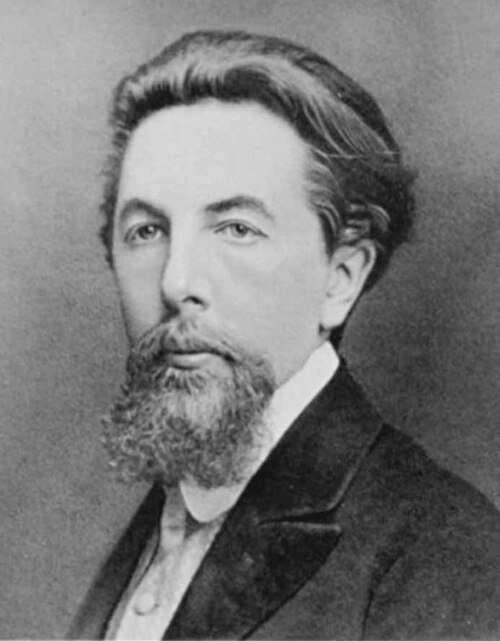
\includegraphics[width=\linewidth]{images/book3/tsvet.jpg}
\end{minipage}\hfill
\begin{minipage}[t]{0.78\linewidth}
\vspace{0pt}
De botanicus Michail Tsvet goot een extract van groene bladeren op een glazen buis gevuld met gepoederd
krijt en spoelde het door met een oplosmiddel: de pigmenten scheidden zich in gekleurde banden, groene
chlorofyllen en gele carotenoïden. In 1906 noemde hij de methode \omterm{def:b2:chromatography:principle}{chromatografie}, ``kleurschrift''.
Ze werd een kwarteeuw lang grotendeels genegeerd, tot ze in de jaren 1930 opnieuw opgepakt werd voor natuurstoffen.
(Portret: onbekende auteur, publiek domein; Wikimedia Commons.)
\end{minipage}
\end{history}

\begin{safety}{\ghs[5mm]{GHS02}\,\ghs[5mm]{GHS05}\,\ghs[5mm]{GHS06}\,\ghs[5mm]{GHS07}\,\ghs[5mm]{GHS08}\,\ghs[5mm]{GHS09}}
Acetonitril en methanol, de gebruikelijke organische componenten van \omterm{def:b2:chromatography:principle}{mobiele fasen} voor HPLC, zijn ontvlambaar en giftig;
hexaan, gebruikt bij kolomchromatografie, is ontvlambaar, schadelijk voor de gezondheid en giftig voor waterorganismen.
Oplosmiddelafval wordt ingezameld, nooit in de gootsteen gegoten.
% ledger: ghs:acetonitrile, ghs:methanol, ghs:hexane
\end{safety}

\section{Oefeningen}

\begin{exercise}[$\star$]\label{exo:b2:chromatography:1}
Een verbinding heeft $t_R = \qty{5.0}{min}$ op een kolom met een \omterm{def:b2:chromatography:retention}{dode tijd} van \qty{1.0}{min}. Bereken haar
\omterm{def:b2:chromatography:retention}{retentiefactor} en de fractie van haar tijd die ze in de \omterm{def:b2:chromatography:principle}{mobiele fase} doorbrengt.
\end{exercise}

\begin{exercise}[$\star$]\label{exo:b2:chromatography:2}
Een piek bij $t_R = \qty{6.0}{min}$ heeft een basisbreedte van \qty{0.30}{min}. Bereken het \omterm{def:b2:chromatography:plates}{schotelgetal}.
\end{exercise}

\begin{exercise}[$\star$]\label{exo:b2:chromatography:3}
Een kolom van \qty{250}{mm} geeft $N = 10\,000$ voor een verbinding. Bereken de \omterm{def:b2:chromatography:plates}{schotelhoogte}.
\end{exercise}

\begin{exercise}[$\star$]\label{exo:b2:chromatography:4}
GC of HPLC? Ethanol in bloed; een eiwit; cafeïne in een drank; benzeen in benzine; suikers in vruchtensap.
\end{exercise}

\begin{exercise}[$\star\star$]\label{exo:b2:chromatography:5}
Twee pieken: $t_{R1} = \qty{4.0}{min}$, $w_1 = \qty{0.40}{min}$; $t_{R2} = \qty{4.6}{min}$, $w_2 =
\qty{0.50}{min}$. Bereken de \omterm{def:b2:chromatography:separation}{resolutie}. Zijn ze tot op de basislijn gescheiden?
\end{exercise}

\begin{exercise}[$\star\star$]\label{exo:b2:chromatography:6}
Hoeveel schotels zijn er nodig om twee verbindingen met $\alpha = 1.10$ en $k_2 = 4.0$ te scheiden bij
$R_s = 1.5$?
\end{exercise}

\begin{exercise}[$\star\star$]\label{exo:b2:chromatography:7}
Een kolom heeft $A = \qty{5}{\micro m}$, $B = \qty{8}{\micro m.mm/s}$, $C = \qty{2}{\micro m.s/mm}$
(gegevens voor de oefening). Zoek de optimale snelheid en de kleinste \omterm{def:b2:chromatography:plates}{schotelhoogte}.
\end{exercise}

\begin{exercise}[$\star\star$]\label{exo:b2:chromatography:8}
Voorspel de elutievolgorde van benzeen, fenol en tolueen bij HPLC met \omterm{def:b2:chromatography:techniques}{omgekeerde fase} en een \omterm{def:b2:chromatography:principle}{mobiele fase}
water--methanol, en wat er gebeurt wanneer de methanolfractie verhoogd wordt.
\end{exercise}

\begin{exercise}[$\star\star$]\label{exo:b2:chromatography:9}
Een ijkoplossing van een analyt bij \qty{20.0}{mg/L} met de \omterm{def:b2:chromatography:quantitative}{interne standaard} bij \qty{10.0}{mg/L}
geeft oppervlakten 860 en 400. Een monster waaraan de standaard is toegevoegd bij \qty{10.0}{mg/L}, geeft oppervlakten 645 en 410.
Bereken de \omterm{def:b2:chromatography:quantitative}{responsfactor} en de concentratie van de analyt (gegevens voor de oefening).
\end{exercise}

\begin{exercise}[$\star\star\star$]\label{exo:b2:chromatography:10}
Een scheiding geeft $R_s = 1.06$. Welke kolomlengte, ten opzichte van de huidige, geeft $R_s = 1.5$, en
wat kost dat aan tijd? Welke andere hefbomen zijn er?
\end{exercise}

\begin{exercise}[$\star\star\star$]\label{exo:b2:chromatography:11}
Bereken voor twee gaussische pieken van gelijke hoogte en breedte met basisbreedte $w = 4\sigma$ het signaal
halverwege ertussen, ten opzichte van de piekhoogte, bij $R_s = 1$ en bij $R_s = 1.5$ (verwaarloos de bijdrage van de verre
piek op elk maximum).
\end{exercise}

\begin{exercise}[$\star\star\star$]\label{exo:b2:chromatography:12}
Vergelijk bij constante $N$ en $\alpha$ de resolutiefactor $k_2/(1+k_2)$ en de relatieve analysetijd
$1 + k_2$ voor $k_2 = 2$, 5 en 10. Welk bereik van $k$ zou je kiezen?
\end{exercise}

\section{Probleem: cafeïne in een energiedrank}

\begin{problem}[{Weekendprobleem --- de elutievolgorde bij omgekeerde fase, de prestaties van een kolom uit een
chromatogram, de scheiding verbeteren, en kwantificering met een interne standaard}]
\label{pb:b2:chromatography:1}
Gegevens voor de oefening (verzonnen, geen echte methode). Een energiedrank wordt tienmaal verdund (\qty{5.00}{mL} tot
\qty{50.0}{mL}) en theofylline wordt als \omterm{def:b2:chromatography:quantitative}{interne standaard} toegevoegd tot \qty{40.0}{mg/L} in de verdunde
oplossing. Kolom: \qty{150}{mm}, \omterm{def:b2:chromatography:techniques}{omgekeerde fase}; \omterm{def:b2:chromatography:principle}{mobiele fase} water--methanol; uv-detectie. De
niet-weerhouden matrix (suikers en zouten) elueert bij $t_M = \qty{1.0}{min}$; theofylline bij
\qty{3.0}{min} (basisbreedte \qty{0.18}{min}); cafeïne bij \qty{3.4}{min} (basisbreedte \qty{0.20}{min}).
IJking: cafeïne \qty{50.0}{mg/L} en theofylline \qty{40.0}{mg/L} geven oppervlakten 1500 en 1000.
Monster: oppervlakten 970 (cafeïne) en 1010 (theofylline). Een blikje bevat \qty{250}{mL}.
% ledger: ghs:caffeine, ghs:methanol

\begin{center}
\begin{tikzpicture}
\begin{axis}[width=0.75\linewidth, height=4.4cm, xmin=0, xmax=5, ymin=0, ymax=1,
  xlabel={tijd (min)}, ylabel={absorbantie (w.e.)}, label style={font=\small},
  tick label style={font=\scriptsize}, ytick=\empty]
\addplot[omDef, thick] table[x=t, y=s] {figdata/out/bachelor-2-chromatogram-c.dat};
\node[font=\scriptsize] at (axis cs:1.0,0.42) {matrix};
\node[font=\scriptsize] at (axis cs:2.62,0.86) {theofylline};
\node[font=\scriptsize] at (axis cs:3.85,0.84) {cafeïne};
\end{axis}
\end{tikzpicture}
\end{center}
% figdata: bachelor-2/chromatogram.py part c

\medskip
\noindent\textbf{Deel I --- \omterm{def:b2:chromatography:techniques}{Omgekeerde fase}.}
\begin{enumerate}
  \item Beschrijf de stationaire en de \omterm{def:b2:chromatography:principle}{mobiele fase} van een kolom met \omterm{def:b2:chromatography:techniques}{omgekeerde fase}.
  \item Waarom elueren de suikers bij de \omterm{def:b2:chromatography:retention}{dode tijd}?
  \item Cafeïne is 1,3,7-trimethylxanthine, theofylline 1,3-dimethylxanthine. Verklaar hun
        elutievolgorde.
  \item Waarom is theofylline hier een goede \omterm{def:b2:chromatography:quantitative}{interne standaard}?
  \item Wat zou er met beide \omterm{def:b2:chromatography:retention}{retentietijden} gebeuren als de methanolfractie verhoogd werd?
  \item Wat meet de \omterm{def:b2:chromatography:retention}{dode tijd}?
\end{enumerate}

\medskip
\noindent\textbf{Deel II --- Prestaties van de kolom.}
\begin{enumerate}[resume]
  \item Bereken de \omterm{def:b2:chromatography:retention}{retentiefactoren} van theofylline en cafeïne.
  \item Bereken de \omterm{def:b2:chromatography:separation}{selectiviteitsfactor}.
  \item Bereken het \omterm{def:b2:chromatography:plates}{schotelgetal} voor cafeïne en voor theofylline.
  \item Bereken de \omterm{def:b2:chromatography:plates}{schotelhoogte} voor cafeïne.
  \item Bereken de \omterm{def:b2:chromatography:separation}{resolutie} tussen de twee pieken.
  \item Controleer ze met de resolutievergelijking.
  \item Zijn de pieken tot op de basislijn gescheiden?
\end{enumerate}

\medskip
\noindent\textbf{Deel III --- Sneller of beter.}
\begin{enumerate}[resume]
  \item Om tijd te winnen, wordt de kolom ingekort tot \qty{75}{mm} (zelfde pakking en debiet). Wat wordt
        de \omterm{def:b2:chromatography:separation}{resolutie}?
  \item En de analysetijd?
  \item Wat zou een kolom van \qty{300}{mm} in plaats daarvan geven, en tegen welke kost?
  \item Welke hefboom werkt in op $\alpha$?
  \item Zou een grotere $k$ hier veel helpen?
\end{enumerate}

\medskip
\noindent\textbf{Deel IV --- Kwantificering.}
\begin{enumerate}[resume]
  \item Bereken de \omterm{def:b2:chromatography:quantitative}{responsfactor} van cafeïne ten opzichte van theofylline.
  \item Waarom doet het geïnjecteerde volume er niet toe?
  \item Bereken de concentratie cafeïne in de verdunde oplossing.
  \item Bereken de concentratie cafeïne in de drank.
  \item Wat zou er misgaan als een verbinding uit de matrix samen met theofylline elueerde?
  \item Wat zou een externe ijking in plaats daarvan vragen?
  \item Geef de massa cafeïne in een blikje van \qty{250}{mL}.
\end{enumerate}
\end{problem}
